\documentclass{article}
\usepackage{graphicx}
\usepackage{tabularx}
\usepackage{booktabs}
\usepackage[raggedrightboxes]{ragged2e}



\title{Problem Statement and Goals for SmartLock\\\progname}

\author{\authname}

\date{\today}

%% Comments
\usepackage{color}
\newif\ifcomments\commentstrue %displays comments
%\newif\ifcomments\commentsfalse %so that comments do not display
\ifcomments
\newcommand{\authornote}[3]{\textcolor{#1}{[#3 ---#2]}}
\newcommand{\todo}[1]{\textcolor{red}{[TODO: #1]}}
\else
\newcommand{\authornote}[3]{}
\newcommand{\todo}[1]{}
\fi
\newcommand{\wss}[1]{\authornote{blue}{SS}{#1}} 
\newcommand{\plt}[1]{\authornote{magenta}{TPLT}{#1}} %For explanation of the template
\newcommand{\an}[1]{\authornote{cyan}{Author}{#1}}
%% Common Parts
\newcommand{\progname}{4TB6 - Mechatronics Capstone} % PUT YOUR PROGRAM NAME HERE
\newcommand{\authname}{Team \#5, Locked \& Loaded
\\ Abi Nevo, nevoa
\\ Elsa Bassi, bassie
\\ Steffi Ralph, ralphs1
\\ Abdul Iqbal, iqbala18
\\ Stephen De Jong, dejons1
\\ Anthony Shenouda, shenoa2} % AUTHOR NAMES                  

\usepackage{hyperref}
    \hypersetup{colorlinks=true, linkcolor=blue, citecolor=blue, filecolor=blue,
                urlcolor=blue, unicode=false}
    \urlstyle{same}


\begin{document}

\bibliographystyle{IEEEtran}
\bibliography{citation}


\maketitle
\thispagestyle{empty}
%\begin{figure}[h!]
  %\centering
  %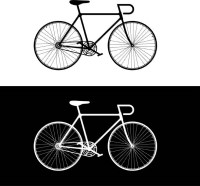
\includegraphics[width=0.4\linewidth]{../BikeLogo.jpg}
%\end{figure}

\newpage
\pagenumbering{roman}
\begin{table}[hp]
\caption{Revision History} \label{TblRevisionHistory}
\begin{tabularx}{\textwidth}{llX}
\toprule
\textbf{Date} & \textbf{Developer(s)} & \textbf{Change}\\
\midrule
25-09-22 & Steffi & Completed\\
19-11-22 & Steffi & Updates for grammar, formatting and terminology\\
23-11-22 & Steffi & Updates for consistency across documentation\\
04-04-23 & Steffi & Final Updates\\
\bottomrule
\end{tabularx}
\end{table}

\newpage
\tableofcontents
\listoftables

\newpage
\pagenumbering{arabic}
\section{Problem Statement}

\subsection{Problem}

There are many problems associated with bike locks today.  People often forget or lose their keys, lock or combination.  Additionally, current locking systems are often not comprehensive – they may not lock all parts of the bike that can be stolen (the seat, front and back wheels and frame). 

Furthermore, the problem stretches beyond the locking mechanisms; bike locks can be bulky, heavy and dangerous to carry around.  The combination of these issues can lead to individuals leaving their bikes without properly locking them.  The city of Toronto reports an average of 3625 stolen bikes annually, and the Canadian Cycling Magazine estimates that only 15-20\% of stolen bikes are reported, indicating a rather expansive problem that needs to be solved [1, 2]. 

Our team presents the SmartLock, which is a bike lock that is unlocked through a smartphone application.  Users can secure their bikes automatically, eliminating the need for manual locking through keys or a combination.  The application includes a geotagging component to locate the bike in case the user forgets where they locked (parked) it.  Additionally, the SmartLock is intended to be mounted permanently on a bike frame, eliminating the need to carry a lock altogether.  The sleek design will ensure that the lock is unobtrusive while riding. 


\subsection{Inputs and Outputs}

\begin{table}[hp]
  \begin{center}
  \caption{Inputs and Outputs} \label{TblTInputsAndOutputs}
    \begin{tabular}{| l | r |}
    \hline
      \textbf{Inputs} & \textbf{Outputs}\\
      \hline
      SignalLock (to lock latch)  & LatchLocked\\
	    SignalUnlock (to unlock) & LatchUnlocked\\
	    SignalOpened & LockOpened\\
	    SignalClosed & LockClosed\\
	    BatteryPower & BatteryPercentStatus\\
	    GeotaggedLocation & BikePosition\\
	    \hline
    \end{tabular}
  \end{center}
\end{table}

\subsection{Stakeholders}

Cyclists or aspiring cyclists who are interested in improving the efficiency, usability and security of locking/finding their bike(s).

\newpage
\subsection{Environment}

Below is a list of the hardware and software needed to implement the solution to the problem.
~\newline
Hardware:
\begin{itemize}
\item Lock Housing - A CAD designed and 3D printed prototype that can house the circuitry and locking mechanism as well as support a chain and connect to the mount
\item Locking Mechanism - A solenoid which when placed inside the housing has the ability to engage/disengage which effectively locks/unlocks the bike
\item SmartLock Mount - A mount that connects to the bike and the lock so that it can be secured to the bike while riding and locked
\item Chain - For external frame locking
\item Battery - To power the circuit
\item Arduino with Bluetooth capabilities - To connect to the app and control the solenoid
\end{itemize}

~\newline
Software: 
\begin{itemize}
\item Smartphone App
\subitem Flutter App UI code
\subitem Integrated C code - To communicate with the Arduino via Bluetooth
\end{itemize}

\newpage
\section{Goals}

\begin{table}[hp]
  \begin{center}
    \caption{Goals} \label{TblGoals}
    \begin{tabular}{| p{0.52\linewidth} | p{0.6\linewidth} |}
    \hline
      \textbf{Goals} & \textbf{Measurability}\\
      \hline
      G1: Wireless communication and \newline engagement/disengagement of bike lock  & Quality and distance of signal strength\\
      \hline
      G2: Effective bike lock: The lock can't be forced open by hand or standard tools.  & Lock functions, X amount of force before failure\\
      \hline
      G3: Long lasting battery life  & Time - in months \\
      \hline
     G4: Fits on many different styles of bikes: Children's, Mountain, Road, and City & Can easily be mounted to mountain bikes, city bikes, children's bikes and road bikes \\
      \hline
      G5: Easily mount on bike frame & Does not require special tools for mount/dismount\\
      \hline
       G6: Cross-platform implementation & Can be used on both an iPhone and an Android smartphone\\
      \hline
    \end{tabular}
  \end{center}
\end{table}

\section{Stretch Goals}
\begin{itemize}
\item Integrating with fitness apps (ie. Strava) for increased capabilities
\item Integrating the battery with a solar panel for self-charging to reduce user interaction with the lock further
\item GPS location services to track the bike if it stolen
\item The locking mechanism shall be able to disengage manually (e.g., with a key/fob), in addition to remotely
\end{itemize}

\newpage
\section{References}

[1]“bicycle-thefts,” data.torontopolice.on.ca. https://data.torontopolice.on.ca/pages/bicycle-thefts (accessed Sep. 25, 2022).
~\newline
[2]L. Hansen-Gillis, “Bike thefts are increasing in Canada: Here’s what you can do to protect your bike,” Canadian Cycling Magazine, Nov. 04, 2020. https://cyclingmagazine.ca/sections/news/bike-theft-canada/ (accessed Sep. 25, 2022).
‌
‌

\end{document}